\documentclass[11pt]{article}
\usepackage[margin=1in]{geometry}
\usepackage{amsmath,amssymb}
\usepackage{booktabs}
\usepackage{multirow}
\usepackage{graphicx}
\usepackage{caption}
\usepackage[hidelinks]{hyperref}
\usepackage{natbib}
\graphicspath{{figures/}}
\captionsetup{font=small,labelfont=bf}
\setlength{\parindent}{0pt}\setlength{\parskip}{0.5em}

\title{\textbf{Learning Dynamics and Market Outcomes\\ in Algorithmic Bertrand Competition}}
\author{Shubh Lamba\\ \small Maharaja Agrasen Institute of Technology, Delhi\\ \small\texttt{lambashubh95@gmail.com}}
\date{\today}

\begin{document}
\maketitle

\begin{abstract}
\noindent We study the pricing behaviour of reinforcement-learning agents in repeated Bertrand
competition with \emph{homogeneous} goods --- the environment in which classical theory predicts the
sharpest competitive outcome. Using $\varepsilon$-greedy Q-learning with state given by rivals'
previous prices, and a stateless mean-based (bandit) benchmark, we run $100$ independent simulations per
configuration and classify outcomes with a Shannon-entropy scheme into competitive, collusive, and
chaotic regimes. Three findings stand out. First, supra-competitive collusion does emerge even in the
homogeneous-goods case --- in $56\%$ of baseline duopoly runs, at roughly half the monopoly markup
($\Delta\approx0.43$) --- but it is \emph{conditional}, not universal: it requires a tractable action
space, annealed exploration, and a sufficiently long horizon, and it collapses into non-convergent
(chaotic) pricing otherwise. Second, and contrary to the intuition that algorithmic sophistication
drives collusion, the \emph{simpler} mean-based learner collude more reliably ($89\%$ of runs) than
Q-learning ($56\%$); the bootstrapped Q-learner is more prone to non-convergence. Third, the intensity
of collusion is governed by the discount factor in a manner consistent with the folk theorem: the
collusion index rises monotonically with patience ($\Delta$ from $0.23$ at $\gamma=0.2$ to $0.45$ at
$\gamma=0.95$). Collusion weakens monotonically as the price grid fines, as exploration persists, as the
horizon shortens, and as a third firm is added. The policy implication is sharpened rather than softened:
tacit algorithmic collusion does not require sophisticated algorithms, but in the hardest competitive
environment it is fragile and condition-dependent.

\medskip
\noindent\textbf{Keywords:} algorithmic collusion, Bertrand competition, reinforcement learning,
Q-learning, tacit collusion, computational economics, competition policy.\\
\textbf{JEL:} D43, L13, L41, C63.
\end{abstract}

\section{Introduction}
The Bertrand model yields one of the sharpest predictions in economic theory: with a homogeneous good and
identical constant marginal costs, the unique Nash equilibrium has all firms pricing at marginal cost and
earning zero profit, so that even a duopoly reproduces the perfectly competitive outcome
\citep{tirole1988}. As firms increasingly delegate pricing to autonomous algorithms, a first-order
question for competition authorities is whether such algorithms can learn to sustain supra-competitive
prices without being instructed to do so \citep{harrington2018,ezrachi2016}.

\citet{calvano2020} showed, in a \emph{differentiated}-product setting, that Q-learning agents converge to
supra-competitive prices and develop reward--punishment strategies. We ask the harder question: does this
occur in the \emph{homogeneous}-goods environment, where the competitive force is strongest and the
Bertrand paradox bites? Picking the hardest case is deliberate: collusion ``even here'' would be a
stronger and more alarming result; the failure of collusion here would delimit the phenomenon.

We implement faithful $\varepsilon$-greedy Q-learning --- with a temporal-difference update, a discount
factor, and state given by rivals' previous prices --- alongside a stateless mean-based (multi-armed
bandit) benchmark, and study $100$ independent runs per configuration. We classify each run into one of
three regimes using a Shannon-entropy measure of price dispersion, and we summarise collusion with a
normalised index $\Delta\in[0,1]$ running from Bertrand--Nash ($0$) to symmetric joint monopoly ($1$).

Our findings revise, rather than echo, the differentiated-goods literature:
\begin{enumerate}\itemsep2pt
\item \textbf{Conditional collusion.} Collusion emerges even with homogeneous goods --- $56\%$ of baseline
duopoly runs, $\Delta\approx0.43$ --- but it is not the universal outcome. The remaining runs are
\emph{chaotic} (non-convergent). Collusion requires a tractable price grid, annealed exploration, and a
long horizon; outside those conditions the dominant outcome is chaos.
\item \textbf{Sophistication is not the driver.} The simple mean-based bandit colludes \emph{more} often
($89\%$) than Q-learning ($56\%$). The temporal-difference bootstrap that defines Q-learning makes
convergence harder here, not easier. Collusion is therefore a generic property of payoff-maximising
learning, not an artefact of algorithmic sophistication.
\item \textbf{Patience governs intensity.} The collusion index rises monotonically with the discount
factor $\gamma$ ($\Delta: 0.23\to0.45$ as $\gamma: 0.2\to0.95$), the comparative static predicted by the
folk theorem.
\item \textbf{Fragility.} Collusion falls monotonically as the grid fines ($57\%\to3\%$), as exploration
persists ($57\%\to0\%$), as the horizon shortens ($57\%\to10\%$), and as a third firm is added
($57\%\to0\%$).
\end{enumerate}

The policy reading is that tacit algorithmic collusion is real and does not require clever algorithms ---
but in the homogeneous-goods limit it lives on a knife-edge of conditions, which both tempers the most
alarmist claims and points to concrete, observable levers (exploration floors, market structure) for
regulation.

\section{Related Literature}
Our work sits at the intersection of classical Bertrand theory, the algorithmic-collusion literature, and
learning in games. The Bertrand paradox \citep{bertrand1883,tirole1988} is relaxed classically by product
differentiation \citep{hotelling1929}, capacity constraints \citep{edgeworth1925}, and repeated
interaction \citep{ivaldi2003}; we study adaptive algorithmic learning as a further channel.
\citet{calvano2020} is the closest antecedent: Q-learning collusion with differentiated products and
reward--punishment strategies. \citet{klein2021} studies sequential pricing; \citet{brown2023} analyse
competition between pricing algorithms; \citet{assad2024} provide empirical evidence from retail gasoline.
On the methodological side, \citet{waltman2008} document that multi-agent Q-learning may cycle rather than
converge --- precisely the chaotic regime we find to be dominant in the homogeneous case ---
and \citet{watkins1992} introduce the algorithm we use. Relative to this literature our contribution is
to (i) push the analysis to the homogeneous-goods limit, (ii) provide an entropy-based regime classifier,
and (iii) show that the \emph{simpler} learner colludes more, reframing collusion as independent of
algorithmic sophistication.

\section{Model}
We consider a repeated Bertrand pricing game with $n\in\{2,3\}$ firms producing a homogeneous good. Each
firm $i$ chooses a price $p_i$ from a finite, evenly spaced grid
\[
\mathcal P=\{p_{\min},\,p_{\min}+\Delta,\,\dots,\,p_{\max}\},\qquad
\Delta=\frac{p_{\max}-p_{\min}}{K-1},\quad K=|\mathcal P|,
\]
with $p_{\min}=0$, $p_{\max}=10$, and a baseline of $K=7$ price points (Section~\ref{sec:robust}
varies $K$). All firms share constant marginal cost $c=1$. Demand is inelastic and normalised to one unit,
allocated by the Bertrand rule
\[
q_i(\mathbf p)=
\begin{cases}
1/\,|\{j:p_j=\min_k p_k\}| & \text{if } p_i=\min_k p_k,\\
0 & \text{otherwise,}
\end{cases}
\qquad \pi_i(\mathbf p)=(p_i-c)\,q_i(\mathbf p).
\]
The stage-game Nash equilibrium is $p_i=c$ for all $i$, with zero profit. Firms interact for $T$ periods
(baseline $T=30{,}000$; Section~\ref{sec:robust} varies $T$). We summarise the degree of collusion by the
index
\[
\Delta=\frac{\bar\pi-\pi^{N}}{\pi^{M}-\pi^{N}},\qquad \pi^{N}=0,\quad \pi^{M}=\frac{p_{\max}-c}{n},
\]
where $\bar\pi$ is the average per-firm per-period profit over the final $T_0=2{,}000$ periods; $\Delta=0$
is Bertrand--Nash and $\Delta=1$ is symmetric joint monopoly.

\section{Learning Algorithms}
\paragraph{Q-learning.} Each firm runs $\varepsilon$-greedy Q-learning \citep{watkins1992}. The state
$s_t$ is the vector of rivals' prices in the previous period; the action is the firm's own price. With
probability $1-\varepsilon$ the firm plays $\arg\max_a Q^i(s_t,a)$, and with probability $\varepsilon$ it
explores uniformly. After observing profit $\pi^i_t$ and the new state $s_{t+1}$, it applies the
temporal-difference update
\begin{equation}
Q^i(s_t,a^i_t)\;\leftarrow\;Q^i(s_t,a^i_t)+\alpha\Big[\pi^i_t+\gamma\max_{a'}Q^i(s_{t+1},a')-Q^i(s_t,a^i_t)\Big],
\label{eq:q}
\end{equation}
with learning rate $\alpha=0.10$ and discount factor $\gamma=0.95$ (baseline). Exploration is annealed,
$\varepsilon_t=\varepsilon_0/(1+\delta t)$ with $\varepsilon_0=0.10$ and $\delta=3\times10^{-4}$;
Section~\ref{sec:robust} compares constant and annealed schedules. Q-tables are initialised at (numerically)
zero. Unlike a bandit, \eqref{eq:q} is forward-looking (through $\gamma\max_{a'}Q$) and state-dependent,
in principle enabling reactive strategies.

\paragraph{Mean-based benchmark.} As a control we use stateless mean-based learning: each agent keeps the
running average payoff of each price, $M^i_t(p)$, and plays $\varepsilon$-greedily with respect to it. This
is a multi-armed bandit: it has no discounting, no state, and no temporal-difference bootstrap. Comparing
the two isolates the role of Q-learning's added machinery.

\section{Behavioural Regimes and Entropy Classification}
Three qualitatively distinct long-run behaviours arise (Figure~\ref{fig:regimes}): a \emph{competitive}
regime with prices near marginal cost and $\Delta\approx0$; a \emph{collusive} regime with both firms
converging to a common supra-competitive price; and a \emph{chaotic} regime of persistent oscillation
without convergence.

\begin{figure}[t]\centering
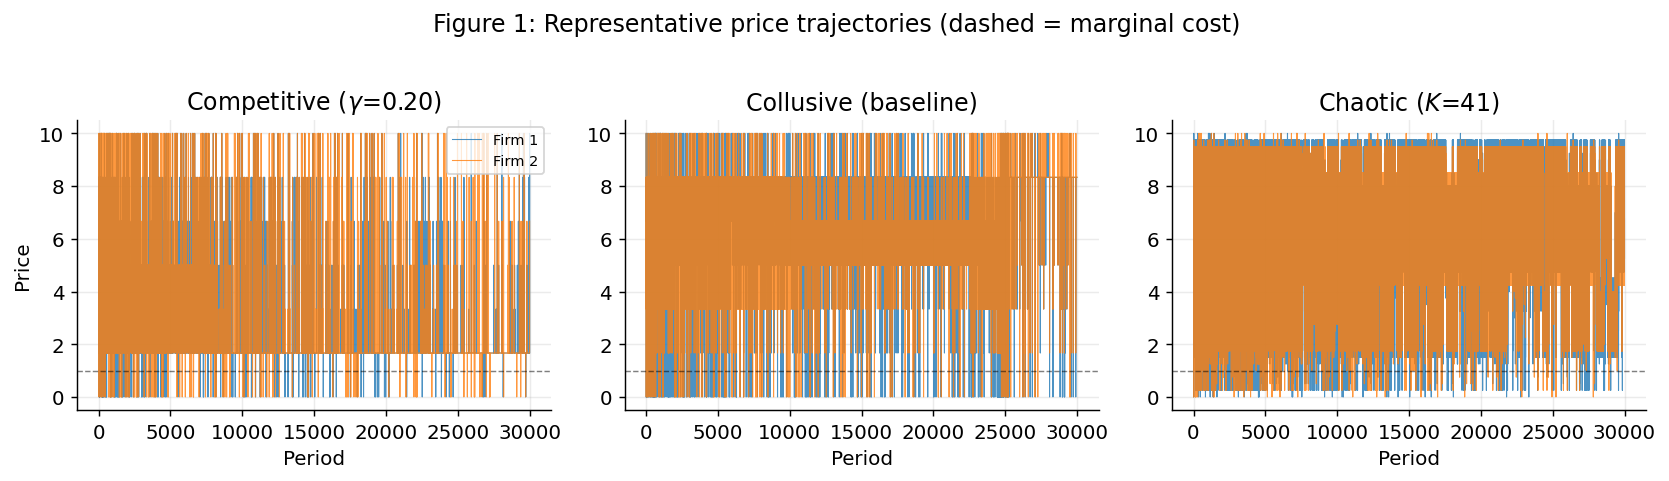
\includegraphics[width=\textwidth]{fig1_regimes.png}
\caption{Representative price trajectories. Left: competitive ($\gamma=0.20$). Centre: collusive
(baseline). Right: chaotic (fine grid, $K=41$). Dashed line is marginal cost $c=1$.}
\label{fig:regimes}
\end{figure}

To classify runs automatically we compute, over the final $T_0$ periods, the empirical price distribution
$f^i(p)$ of each agent and its Shannon entropy $H^i=-\sum_p f^i(p)\log_2 f^i(p)$, averaged to
$\bar H=\frac1n\sum_i H^i$. Writing $\bar p$ for the mean price over the window, the regime is
\[
\text{Regime}=
\begin{cases}
\text{Competitive} & \bar H<H^\ast \text{ and } \bar p<p^\ast,\\
\text{Collusive} & \bar H<H^\ast \text{ and } \bar p\ge p^\ast,\\
\text{Chaotic} & \bar H\ge H^\ast,
\end{cases}
\qquad H^\ast=1.0,\ p^\ast=2.0.
\]
Entropy distinguishes converged play (low $\bar H$) from non-convergent play (high $\bar H$); mean price
then separates competitive from collusive convergence. Figure~\ref{fig:map} shows the $100$ baseline runs
in the $(\bar H,\bar p)$ plane, with the two clusters --- a converged collusive mass and a high-entropy
chaotic mass --- clearly separated by $H^\ast$.

\begin{figure}[t]\centering
\begin{minipage}{0.49\textwidth}\centering
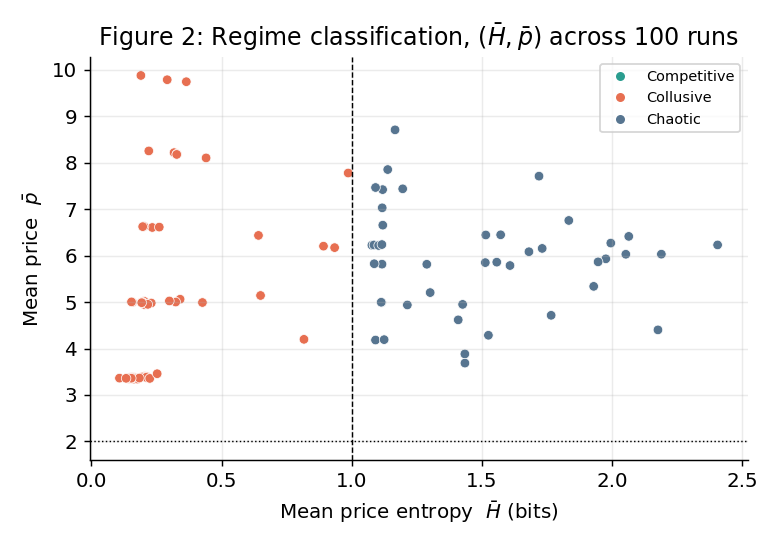
\includegraphics[width=\textwidth]{fig2_regime_map.png}
\caption{Regime classification of $100$ baseline runs in $(\bar H,\bar p)$.}
\label{fig:map}
\end{minipage}\hfill
\begin{minipage}{0.49\textwidth}\centering
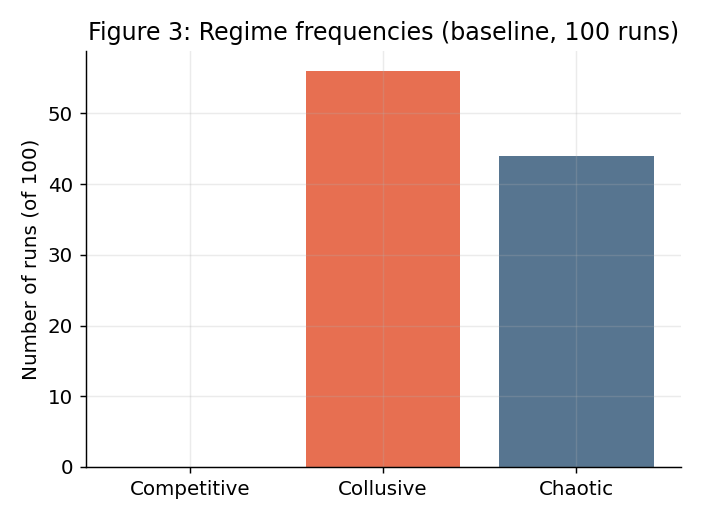
\includegraphics[width=\textwidth]{fig3_regime_freq.png}
\caption{Baseline regime frequencies (of $100$ runs).}
\label{fig:freq}
\end{minipage}
\end{figure}

\section{Baseline Results}
Under the baseline duopoly configuration, $56\%$ ($\pm5.0$) of runs are collusive and $44\%$ chaotic;
competitive convergence essentially never occurs (Figure~\ref{fig:freq}). The mean collusion index is
$\Delta=0.43$, i.e.\ converged runs sit roughly half-way between marginal-cost pricing and joint monopoly.
The distribution of mean prices (Figure~\ref{fig:dist}) is bimodal: a mass of converged collusive runs at
high prices and a spread of chaotic runs at intermediate prices, with almost no mass at marginal cost.
Thus collusion is the single most common \emph{converged} outcome, but non-convergence is nearly as
likely: in the homogeneous-goods limit, learning to collude and failing to settle are comparably probable.

\begin{figure}[t]\centering
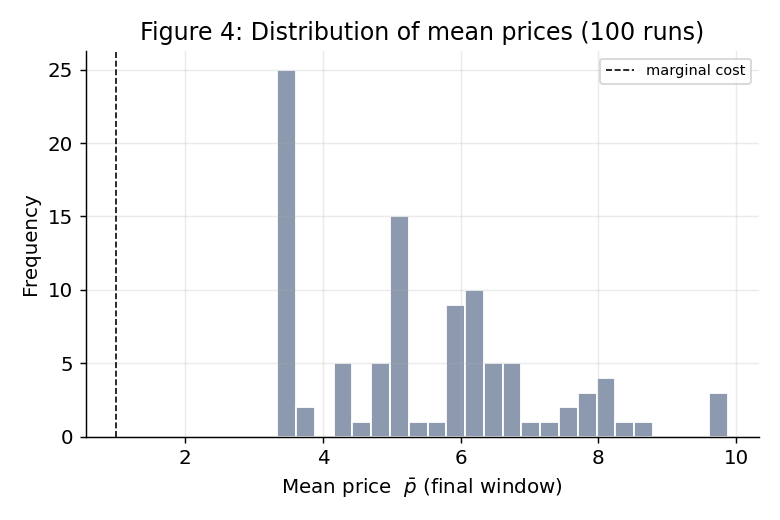
\includegraphics[width=0.62\textwidth]{fig4_price_dist.png}
\caption{Distribution of mean prices across $100$ baseline runs (dashed line: marginal cost).}
\label{fig:dist}
\end{figure}

\section{Q-learning versus Mean-Based Learning}
Comparing the two algorithms under identical conditions yields our most counterintuitive result
(Figure~\ref{fig:qvm}): the stateless mean-based bandit colludes in $89\%$ of runs, against only $56\%$
for Q-learning. The added sophistication of Q-learning --- the temporal-difference bootstrap and the
enlarged state space --- makes convergence \emph{harder}, not easier, so a larger share of Q-learning runs
end chaotic. Mean-based agents, by contrast, settle quickly onto the price with the highest historical
average payoff, which under symmetric play is supra-competitive, and stay there.

This reverses the natural hypothesis that collusion is a product of algorithmic sophistication. In the
homogeneous-goods environment, collusion is if anything the \emph{default} of naive payoff-averaging, and
the more elaborate learner is more easily destabilised. For competition policy this is the more
uncomfortable reading: supra-competitive coordination does not require firms to deploy advanced
reinforcement learning; a simple bandit suffices.

\begin{figure}[t]\centering
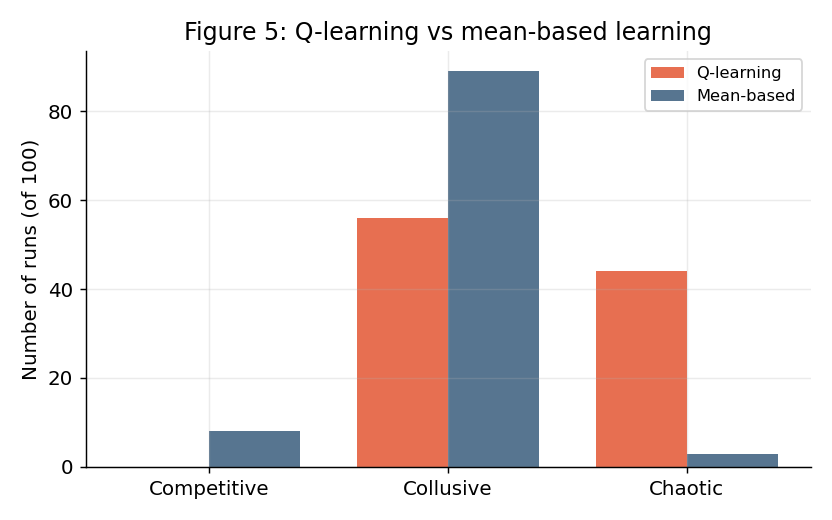
\includegraphics[width=0.6\textwidth]{fig5_q_vs_mean.png}
\caption{Regime frequencies under Q-learning versus mean-based learning ($100$ runs each).}
\label{fig:qvm}
\end{figure}

\section{Patience and the Intensity of Collusion}
The discount factor $\gamma$ governs how heavily an agent weighs future payoffs, and hence its willingness
to forgo a one-period undercut to preserve an ongoing arrangement. Consistent with the folk theorem
\citep{tirole1988}, the intensity of collusion rises monotonically with patience: the mean collusion index
climbs from $\Delta=0.23$ at $\gamma=0.20$ to $\Delta=0.45$ at $\gamma=0.95$ (Figure~\ref{fig:gamma}).
Impatient agents ($\gamma=0.20$) still coordinate frequently but only weakly, and are the only setting in
which the competitive regime appears with non-trivial probability; patient agents collude more intensely
but, because they pursue higher and more fragile prices, also fall into chaos more often. The Q-learner
thus discovers folk-theorem-like behaviour through adaptive search, with $\gamma$ playing the role of
patience --- without any knowledge of repeated-game theory.

\begin{figure}[t]\centering
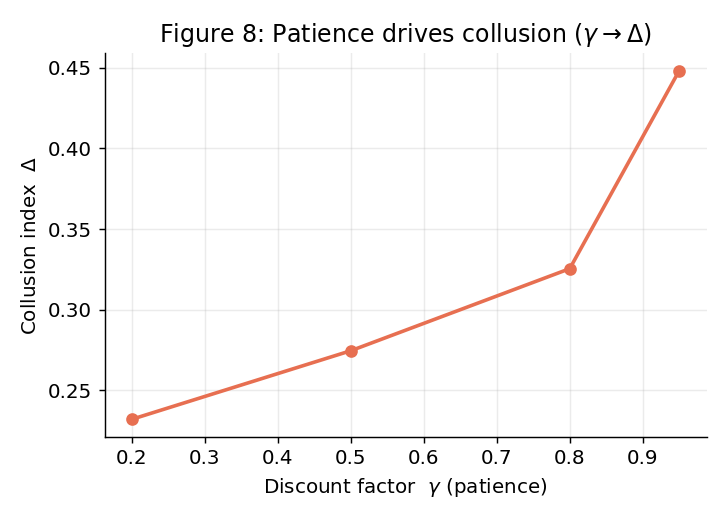
\includegraphics[width=0.58\textwidth]{fig8_gamma_delta.png}
\caption{Collusion index $\Delta$ as a function of the discount factor $\gamma$ (patience).}
\label{fig:gamma}
\end{figure}

\section{Robustness and the Fragility of Collusion}\label{sec:robust}
Table~\ref{tab:sens} reports the share of collusive runs and the mean collusion index as we vary, one at a
time, the discount factor, exploration schedule, grid granularity, horizon, and number of firms ($30$ runs
per cell). Four comparative statics emerge sharply, all in the direction theory predicts.

\begin{table}[t]\centering\small
\caption{Sensitivity analysis. Collusive share ($\%$ of $30$ runs) and mean collusion index $\Delta$.
Baseline: $n{=}2$, $K{=}7$, $\gamma{=}0.95$, annealed $\varepsilon$, $T{=}30{,}000$.}
\label{tab:sens}
\begin{tabular}{llcc}
\toprule
Parameter & Value & Collusive (\%) & $\Delta$ \\
\midrule
\multirow{4}{*}{Discount $\gamma$}
 & $0.20$ & $83$ & $0.23$\\
 & $0.50$ & $97$ & $0.27$\\
 & $0.80$ & $93$ & $0.33$\\
 & $0.95$ (base) & $57$ & $0.45$\\
\midrule
\multirow{3}{*}{Exploration $\varepsilon$}
 & annealed (base) & $57$ & $0.45$\\
 & constant $0.10$ & $13$ & $0.32$\\
 & constant $0.30$ & $0$ & $0.23$\\
\midrule
\multirow{4}{*}{Grid $K$}
 & $7$ (base) & $57$ & $0.45$\\
 & $11$ & $10$ & $0.33$\\
 & $21$ & $3$ & $0.33$\\
 & $41$ & $3$ & $0.30$\\
\midrule
\multirow{4}{*}{Horizon $T$}
 & $5{,}000$ & $10$ & $0.33$\\
 & $15{,}000$ & $30$ & $0.39$\\
 & $30{,}000$ (base) & $57$ & $0.45$\\
 & $60{,}000$ & $77$ & $0.49$\\
\midrule
\multirow{2}{*}{Firms $n$}
 & $2$ (base) & $57$ & $0.45$\\
 & $3$ & $0$ & $0.23$\\
\bottomrule
\end{tabular}
\end{table}

\paragraph{Grid granularity.} Collusion is highly sensitive to the size of the action space: the collusive
share falls from $57\%$ at $K=7$ to $3\%$ at $K=41$. A finer grid enlarges the state--action space faster
than agents can learn it within the horizon, so the dominant outcome becomes chaotic. This is the central
reason a naive ``fine grid, short horizon'' specification finds no collusion at all.

\paragraph{Exploration.} Annealing exploration is necessary for stable collusion. With constant
$\varepsilon=0.10$ the collusive share is only $13\%$, and with $\varepsilon=0.30$ it is zero: persistent
random perturbation repeatedly destabilises any incipient arrangement. The natural tendency of an efficient
algorithm to reduce exploration as it grows confident is therefore precisely the feature that enables
collusion --- and a mandated exploration floor is a candidate pro-competitive intervention.

\paragraph{Horizon.} Collusion rises monotonically with the horizon ($10\%$ at $T=5{,}000$ to $77\%$ at
$T=60{,}000$), confirming that short-horizon specifications understate collusion simply because learning
has not converged.

\paragraph{Market structure.} Adding a third firm collapses collusion entirely ($57\%\to0\%$, all runs
chaotic): the joint state space grows combinatorially and the incentive to undercut two rivals rises,
making coordination far more fragile. Figure~\ref{fig:three} illustrates a representative three-firm run.

\begin{figure}[t]\centering
\begin{minipage}{0.42\textwidth}\centering
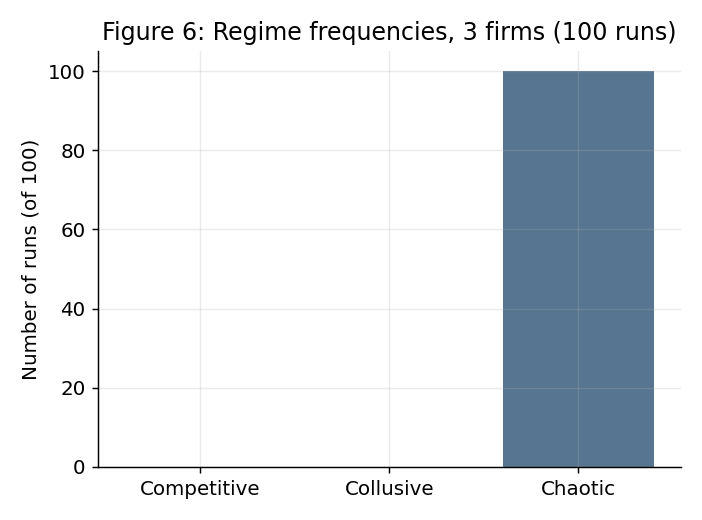
\includegraphics[width=\textwidth]{fig6_three_firm.png}
\caption{Regime frequencies with three firms ($100$ runs).}
\label{fig:three}
\end{minipage}\hfill
\begin{minipage}{0.55\textwidth}\centering
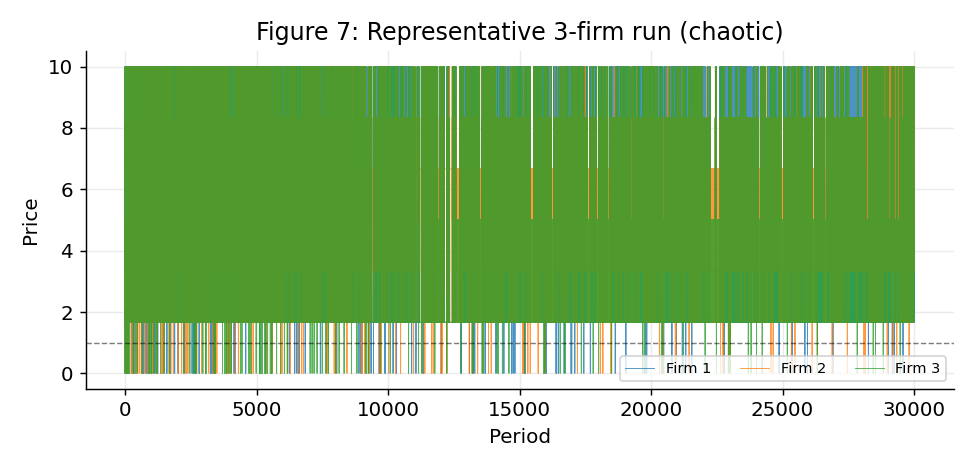
\includegraphics[width=\textwidth]{fig7_three_firm_run.png}
\caption{Representative three-firm price trajectory (chaotic).}
\label{fig:threerun}
\end{minipage}
\end{figure}

\section{Discussion}
Three implications follow. First, the Bertrand paradox is not robust to adaptive learning even with
homogeneous goods: payoff-maximising algorithms reach supra-competitive prices in a majority of converged
runs, with no communication or instruction to collude. Second, because the \emph{simpler} learner colludes
more, the phenomenon is not a quirk of advanced reinforcement learning; it is a generic tendency of
independent payoff optimisation, which broadens rather than narrows the policy concern. Third, however, in
the homogeneous-goods limit collusion is fragile and condition-dependent --- it requires a tractable action
space, annealed exploration, a long horizon, and few firms --- so the differentiated-goods alarm of
\citet{calvano2020} should be read as an upper bound on how easily algorithmic collusion arises.

For enforcement, the conduct-based framework that requires evidence of agreement is ill-suited to a setting
where coordination emerges from independent learning with no communication \citep{harrington2018,ezrachi2016}.
Our results point to observable, structural levers: exploration floors (which we find directly prevent
convergence to collusion), market-structure thresholds (collusion vanishes at three firms), and the
coarseness of admissible price grids.

\paragraph{Limitations.} The analysis is computational and offers no convergence proofs; multi-agent
Q-learning is known to cycle rather than converge in general \citep{waltman2008}, which our chaotic regime
reflects. We restrict attention to homogeneous goods, inelastic demand, tabular learners, and memory-one
state; richer demand, deep reinforcement learning, and longer memory are natural extensions. The collusive
share depends on the entropy threshold $H^\ast$ and price threshold $p^\ast$; we report the comparative
statics, which are robust to moderate threshold changes, rather than treating any single frequency as
exact.

\section{Conclusion}
Implementing faithful Q-learning and a mean-based benchmark in homogeneous-good Bertrand competition, we
find that supra-competitive collusion does emerge --- in a majority of converged duopoly runs, at about
half the monopoly markup --- but that it is conditional rather than universal, that it does not require
algorithmic sophistication (a simple bandit colludes more), that its intensity tracks patience as the folk
theorem predicts, and that it collapses under fine price grids, persistent exploration, short horizons, or
additional firms. Tacit algorithmic collusion is thus both more accessible (it needs no clever algorithm)
and more fragile (it lives on a knife-edge of conditions) than a reading of the differentiated-goods
literature alone would suggest.

\paragraph{Reproducibility.} All code, data, and figure-generating scripts are available at
\url{https://github.com/shubhL-research/algorithmic-bertrand-rl}; every result is produced from fixed
random seeds by a single script.

\bibliographystyle{plainnat}
\begin{thebibliography}{99}
\bibitem[Assad et al.(2024)]{assad2024} Assad, S., Clark, R., Ershov, D., Xu, L. (2024). Algorithmic pricing and competition: Empirical evidence from the German retail gasoline market. \emph{Journal of Political Economy} 132(3), 723--771.
\bibitem[Bertrand(1883)]{bertrand1883} Bertrand, J. (1883). Th\'eorie math\'ematique de la richesse sociale. \emph{Journal des Savants} 67, 499--508.
\bibitem[Brown and MacKay(2023)]{brown2023} Brown, Z.Y., MacKay, A. (2023). Competition in pricing algorithms. \emph{American Economic Journal: Microeconomics} 15(2), 109--156.
\bibitem[Calvano et al.(2020)]{calvano2020} Calvano, E., Calzolari, G., Denicol\`o, V., Pastorello, S. (2020). Artificial intelligence, algorithmic pricing, and collusion. \emph{American Economic Review} 110(10), 3267--3297.
\bibitem[Edgeworth(1925)]{edgeworth1925} Edgeworth, F.Y. (1925). \emph{Papers Relating to Political Economy}, vol.\ 1. Macmillan.
\bibitem[Ezrachi and Stucke(2016)]{ezrachi2016} Ezrachi, A., Stucke, M.E. (2016). \emph{Virtual Competition}. Harvard University Press.
\bibitem[Harrington(2018)]{harrington2018} Harrington, J.E. (2018). Developing competition law for collusion by autonomous price-setting agents. \emph{Journal of Competition Law \& Economics} 14(3), 331--363.
\bibitem[Hotelling(1929)]{hotelling1929} Hotelling, H. (1929). Stability in competition. \emph{Economic Journal} 39(153), 41--57.
\bibitem[Ivaldi et al.(2003)]{ivaldi2003} Ivaldi, M., Jullien, B., Rey, P., Seabright, P., Tirole, J. (2003). The economics of tacit collusion. IDEI Working Paper.
\bibitem[Klein(2021)]{klein2021} Klein, T. (2021). Autonomous algorithmic collusion: Q-learning under sequential pricing. \emph{RAND Journal of Economics} 52(3), 538--558.
\bibitem[Tirole(1988)]{tirole1988} Tirole, J. (1988). \emph{The Theory of Industrial Organization}. MIT Press.
\bibitem[Waltman and Kaymak(2008)]{waltman2008} Waltman, L., Kaymak, U. (2008). Q-learning agents in a Cournot oligopoly model. \emph{Journal of Economic Dynamics and Control} 32(10), 3275--3293.
\bibitem[Watkins and Dayan(1992)]{watkins1992} Watkins, C.J.C.H., Dayan, P. (1992). Q-learning. \emph{Machine Learning} 8(3--4), 279--292.
\end{thebibliography}

\end{document}
